\documentclass{beamer}
\usepackage{ctex, hyperref}
\usepackage[T1]{fontenc}

% other packages
\usepackage{latexsym,amsmath,xcolor,multicol,booktabs,calligra}
\usepackage{graphicx,pstricks,listings,stackengine}

\author{匿名}
\title{基于可信执行环境的高性能加密重复数据删除研究}
\subtitle{硕士学位论文答辩}
\institute{电子科技大学计算机科学与工程学院(网络空间安全学院)}
\date{2022年5月13日}
\usepackage{UESTC}

% defs
\def\cmd#1{\texttt{\color{red}\footnotesize $\backslash$#1}}
\def\env#1{\texttt{\color{blue}\footnotesize #1}}
\definecolor{deepblue}{rgb}{0,0,0.5}
\definecolor{deepred}{rgb}{0.6,0,0}
\definecolor{deepgreen}{rgb}{0,0.5,0}
\definecolor{halfgray}{gray}{0.55}

\lstset{
    basicstyle=\ttfamily\small,
    keywordstyle=\bfseries\color{deepblue},
    emphstyle=\ttfamily\color{deepred},    % Custom highlighting style
    stringstyle=\color{deepgreen},
    numbers=left,
    numberstyle=\small\color{halfgray},
    rulesepcolor=\color{red!20!green!20!blue!20},
    frame=shadowbox,
}

\newcommand{\sysnameS}{TEEDedup }
\newcommand{\sysnameF}{FeatureSpy }
\newcommand{\prototype}{TEEDedup+ }

\begin{document}

\kaishu
\begin{frame}
    \titlepage
\end{frame}

% \begin{frame}
%     \tableofcontents[sectionstyle=show,subsectionstyle=show/shaded/hide,subsubsectionstyle=show/shaded/hide]
% \end{frame}


\section{研究背景}

% \begin{frame}{外包数据存储}
%     \begin{itemize}[<+-| alert@+>] % 当然,除了alert,手动在里面插 \pause 也行
%         \item Outsourcing data management to cloud is common in practice
%         \item 22% business data are stored in the cloud[*]
%         \item  Outsourcing storage should fulfill security and storage efficiency
%         \item  Security: protect outsourced data against unauthorized access
%         \item  Storage efficiency: reduce storage footprints
%     \end{itemize}
% \end{frame}

\begin{frame}{外包数据存储}
    \begin{itemize}
        \item Outsourcing data management to cloud is common in practice
              \begin{itemize}
                  \item 22\% business data are stored in the cloud[*]
              \end{itemize}
        \item  Outsourcing storage should fulfill security and storage efficiency
              %   \vspace{-1em}
              \begin{itemize}
                  \item  Security: protect outsourced data against unauthorized access
                  \item  Storage efficiency: reduce storage footprints
              \end{itemize}
    \end{itemize}
\end{frame}

\section{研究内容}

\begin{frame}{如何使用块}
    \begin{block}{块的名称}
        \begin{itemize}
            \item A
            \item B
        \end{itemize}
    \end{block}
\end{frame}

\begin{frame}{如何使用定义、定理、引理、证明}

    \kaishu
    \begin{define}[定义名称]
        定义内容
    \end{define}

    \begin{lem}[引理名称]
        引理内容
    \end{lem}

    \begin{thm}[定理名称]
        定理内容(这里的定义、引理、定理分章节自动标号)
    \end{thm}

    \begin{proof}
        证明内容
    \end{proof}

\end{frame}

\begin{frame}[fragile]
    \begin{columns}
        \column{.6\textwidth}
        \begin{lstlisting}[language=TeX]
    \begin{table}[htbp]
      \caption{编号与含义}
      \label{tab:number}
      \centering
      \begin{tabular}{cl}
        \toprule
        编号 & 含义 \\
        \midrule
        1 & 4.0 \\
        2 & 3.7 \\
        \bottomrule
      \end{tabular}
    \end{table}
    公式~(\ref{eq:vsphere}) 的
    编号与含义请参见
    表~\ref{tab:number}。
\end{lstlisting}
        \column{.4\textwidth}
        \begin{table}[htpb]
            \centering
            \caption{编号与含义}
            \label{tab:number}
            \begin{tabular}{cl}\toprule
                编号 & 含义 \\\midrule
                1    & 4.0  \\
                2    & 3.7  \\\bottomrule
            \end{tabular}
        \end{table}
        \normalsize 公式~(\ref{eq:vsphere})的编号与含义请参见表~\ref{tab:number}。
    \end{columns}
\end{frame}



\section{实验分析}

\subsection{实验环境}

\begin{frame}{测试环境与数据集}
    \begin{textbox}{测试数据集}
        \vspace{-1em}
        \begin{table}[!htb]
            \small
            \centering
            \caption{真实世界数据集的特征}
            \label{tab:featurespy-datasets}
            \begin{tabular}{cccc}
                \toprule
                {\bf 数据集} & {\bf 快照总数} & {\bf 去重前总数据量} & {\bf 重复数据删除系数} \\
                \midrule
                FSL          & 795            & 56.2\,TiB            & 140.4                  \\
                MS           & 143            & 14.4\,TiB            & 6.0                    \\
                Linux        & 84             & 44.9\,GiB            & 1.3                    \\
                CouchDB      & 83             & 22.9\,GiB            & 1.5                    \\
                \bottomrule
            \end{tabular}
        \end{table}
    \end{textbox}

    \begin{textbox}{测试平台}
        \begin{itemize}
            \item 本地集群(LAN)。万兆局域网内多台Intel SGX设备,每台设备均采用Intel Core i7-10700 CPU,4\,TB SATA机械硬盘,32\,GB DDR4内存
            \item 云环境(Cloud)。在两个不同区域的阿里云部署了多台规格为\textit{ecs.g7t.3xlarge}的虚拟机(VM)来分别运行云服务端、密钥服务器和多个客户端。
        \end{itemize}
    \end{textbox}
\end{frame}

\subsection{\sysnameS 原型系统}

\begin{frame}{密钥生成效率}
    \begin{figure}[htpb]
        \centering
        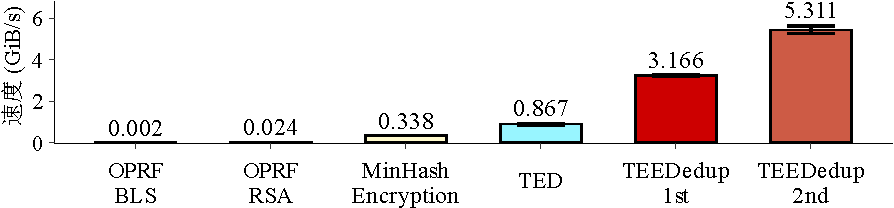
\includegraphics[width=\linewidth]{../pic/sgxdedup/plot/exp_a2/expa2_keyGenPerformance.pdf}
        \caption{单客户端密钥生成性能对比}
    \end{figure}

    \begin{itemize}
        \item TEEDedup提出的密钥生成方案相比OPRF-BLS和OPRF-RSA在第一轮(不含推测性加密)中实现了1,583倍和131.9倍的性能提升,而第二轮基于推测性加密,TEEDedup将第一轮的密钥生成速度再次提高了67.8\%
    \end{itemize}
\end{frame}

% \begin{frame}{会话密钥更新开销}
%     \begin{figure}[!htb]
%         \centering
%         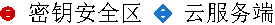
\includegraphics[height=11pt]{../pic/sgxdedup/plot/exp_a5/expa5_keyRegression_time_legend.pdf}
%         \begin{tabular}{@{\ }c@{\ }c}
%             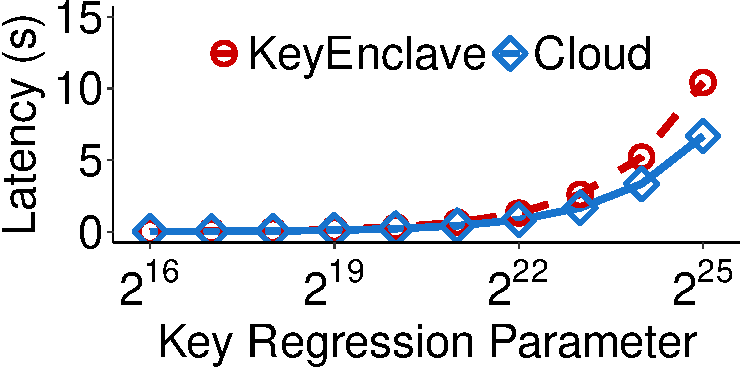
\includegraphics[width=0.49\textwidth]{../pic/sgxdedup/plot/exp_a5/expa5_keyRegression_time.pdf} &
%             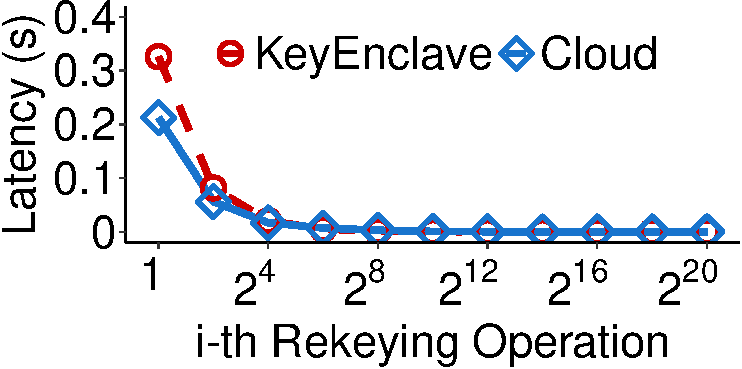
\includegraphics[width=0.49\textwidth]{../pic/sgxdedup/plot/exp_a5/expa5_keyRegression_time_default.pdf} \\
%             \mbox{\small (a)密钥回归参数的影响}                                                              &
%             \mbox{\small (b)密钥回归执行次数的影响}
%         \end{tabular}
%         \caption{会话密钥更新延迟}
%         \label{fig:sgxdedup-rekeyingLatency}
%     \end{figure}
%     \begin{itemize}
%         \item 密钥更新开销较低:密钥安全区的密钥更新延迟为0.040\,s,云服务端约为0.027\,s。
%         \item 安全区处理密集计算的能力较弱,其密钥更新延迟相较云服务端高1.22~1.56倍。
%     \end{itemize}
% \end{frame}

\begin{frame}{数据块所有权证明效率}
    \begin{figure}[!htb]
        \begin{minipage}[t]{0.47\textwidth}
            \centering
            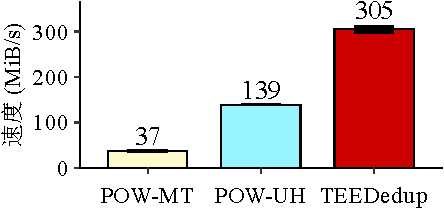
\includegraphics[width=\linewidth]{../pic/sgxdedup/plot/exp_a4/expa4_powPerformance.pdf}
            \caption{数据所有权证明的计算性能(不含网络开销)}
            \label{fig:sgxdedup-pow-comparison}
        \end{minipage}%
        \hspace{0.2in}
        \begin{minipage}[t]{0.47\textwidth}
            \centering
            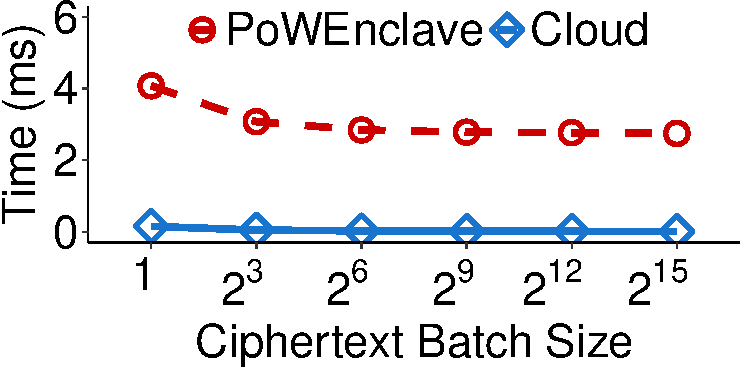
\includegraphics[width=\linewidth]{../pic/sgxdedup/plot/exp_a4/expa4_powBatchSize_breakdown.pdf}
            \caption{所有权证明的计算开销vs.批量大小(单位:ms/MiB)}
            \label{fig:sgxdedup-multiClientThroughput}
        \end{minipage}%
    \end{figure}
    \begin{itemize}
        \item 由于\sysnameS 避免了客户端中的纠删码编码和Merkle树构造,实现了相较于PoW-MT 8.2倍的性能提升。相较于安全性较弱的PoW-UH实现了2.2倍的性能提升。
        \item 云服务端的计算时间开销很低(低于0.05\,ms),而所有权证明安全区的计算时间随着批量大小增大从4.1\,ms减少到 2.7\,ms。
    \end{itemize}
\end{frame}

\begin{frame}{\sysnameS 原型系统性能}
    \begin{figure}[!htb]
        \centering
        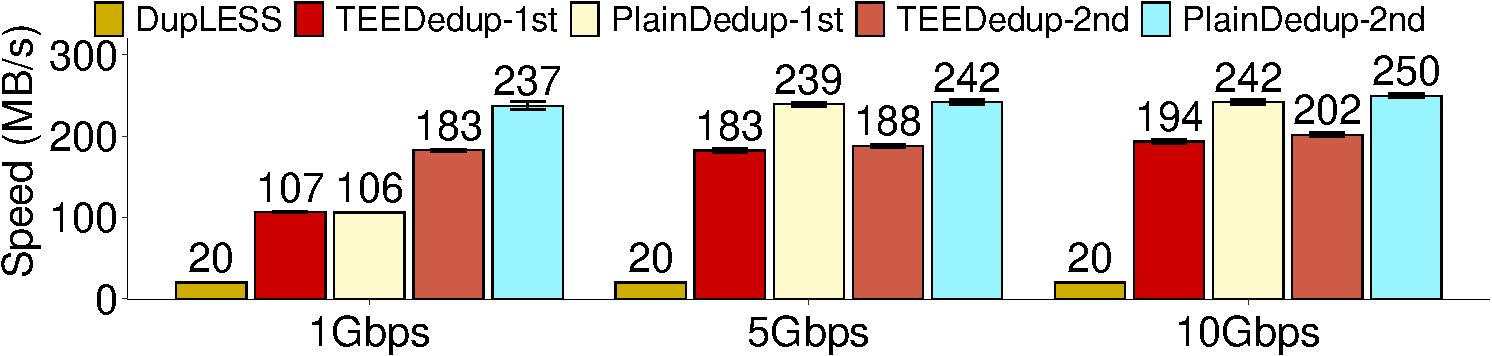
\includegraphics[width=0.646\textwidth]{../pic/sgxdedup/plot/exp_b1/upload_network_speed_bar.pdf}
        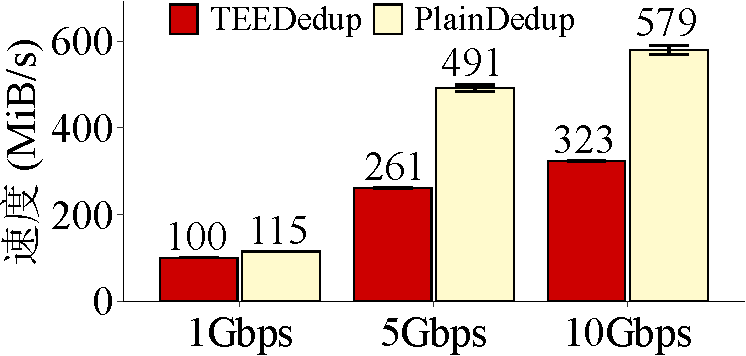
\includegraphics[width=0.324\textwidth]{../pic/sgxdedup/plot/exp_b1/download_network_speed_bar.pdf}
        \\
        \hspace{1.1in} {\small (a) 上传} \hspace{1.4in}
        {\small (b) 下载}\\
        \caption{单客户端在不同网络速度下的上传/下载性能}
        \label{fig:sgxdedup-singleClientThroughput}
    \end{figure}

    \begin{itemize}
        \item \sysnameS 在第一轮和第二轮上传中分别相对DupLESS实现了8.1倍和9.6倍的性能提升。
        \item 与不安全的PlainDedup相比,\sysnameS 仅导致两轮上传速度分别下降约17.5\%和21.4\%。
    \end{itemize}
\end{frame}

\subsection{\sysnameF 检测方案}

\begin{frame}{密文数据块的相似性检测}
    \begin{columns}
        \begin{column}{.5\textwidth}
            \vspace{-1em}
            \begin{figure}[!htb]
                \centering
                
\includegraphics[width=0.8\linewidth]{../pic/featurespy/plot/detection/syn/synBarPlotDetect_legend.pdf}\\
                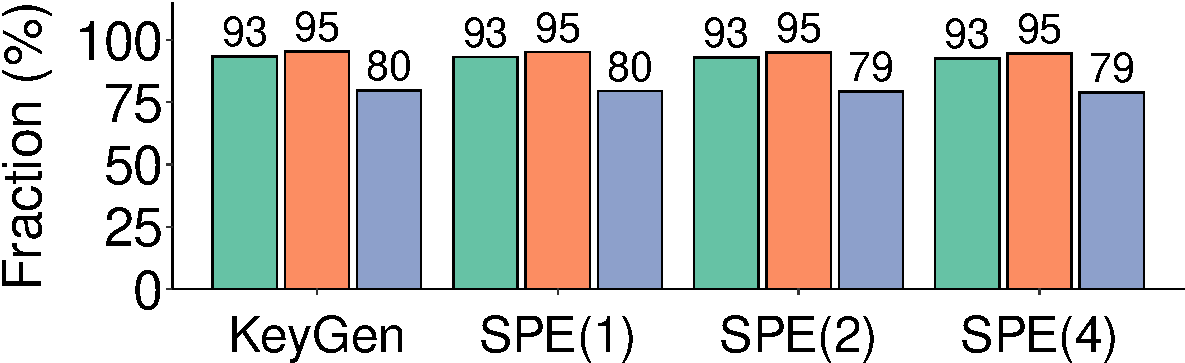
\includegraphics[width=\linewidth]{../pic/featurespy/plot/detection/syn/syn-p1-q4-detect.pdf}  \\
                \vspace{-3pt}
                \mbox{\fontsize{8.0pt}{\baselineskip}\selectfont (a) $\textrm{SYNChunk}(1, 4)$}                                                        \\
                \vspace{-3pt}
                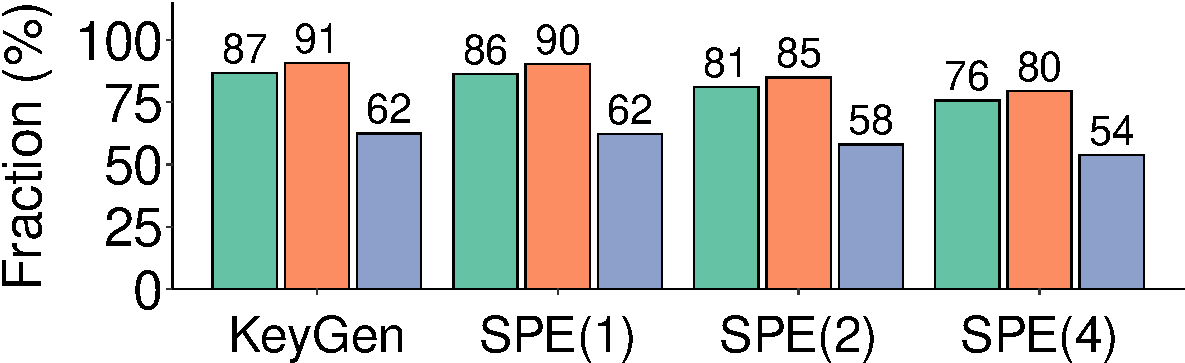
\includegraphics[width=\linewidth]{../pic/featurespy/plot/detection/syn/syn-p2-q8-detect.pdf}    \\
                \vspace{-3pt}
                \mbox{\fontsize{8.0pt}{\baselineskip}\selectfont (b) $\textrm{SYNChunk}(2, 8)$}                                                          \\
                \vspace{-3pt}
                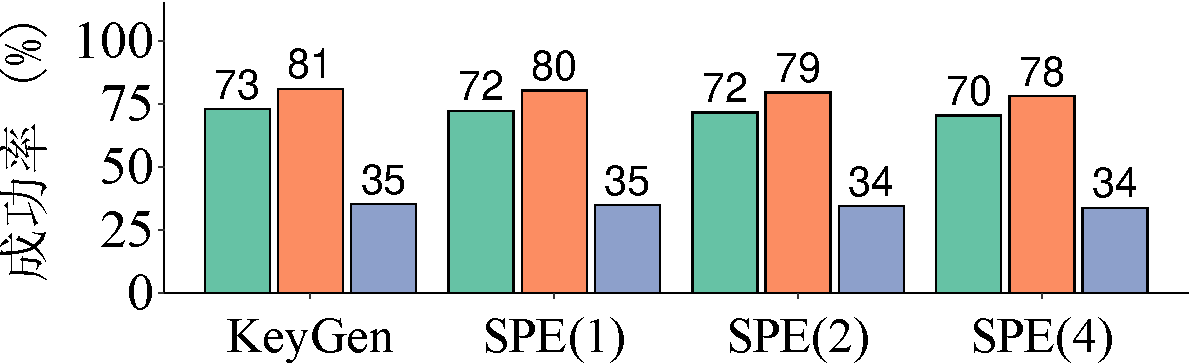
\includegraphics[width=\linewidth]{../pic/featurespy/plot/detection/syn/syn-p4-q16-detect.pdf} \\
                \vspace{-3pt}
                \mbox{\fontsize{8.0pt}{\baselineskip}\selectfont (c) $\textrm{SYNChunk}(4, 16)$}                                                       \\
                \vspace{-3pt}
                \caption{密文数据块的相似性检测效果}
                \label{fig:featurespy-expDetectionSynDetect}
            \end{figure}
        \end{column}
        \begin{column}{.5\textwidth}
            \begin{itemize}
                \item {\tt minFeature}方案对数据块内容的随机变化更不敏感。
                \item 相似性保留加密在加密后保留了较高的相似性: 通过检查密文数据块中的相似性指标,在SYNChunk$(1,4)$、SYNChunk$(2,8)$、SYNChunk$(4,16)$数据集中分别检测到至多95.2\%、90.4\%、80.2\%的相似数据块。
            \end{itemize}
        \end{column}
    \end{columns}
\end{frame}

\begin{frame}{推测内容攻击检测效果案例分析}
    \begin{columns}
        \begin{column}{.6\textwidth}
            \vspace{-1em}
            \begin{figure}[!htb]
                \centering
                
\includegraphics[width=\linewidth]{../pic/featurespy/plot/detection/overall/prefixDistribution_legend.pdf}\\
                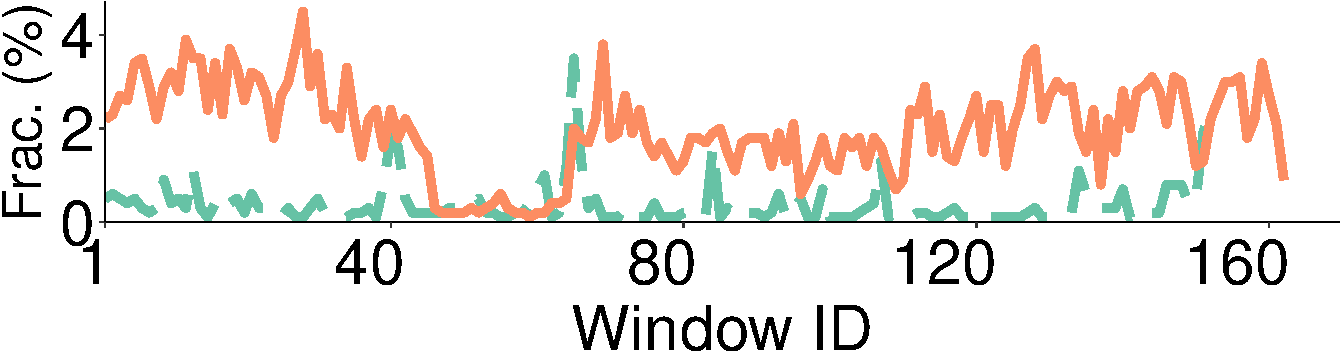
\includegraphics[width=\linewidth]{../pic/featurespy/plot/detection/overall/prefixDistribution-1000-Linux-min.pdf}\\
                \caption{Linux最新快照在包含/不包含攻击行为时每个窗口(W=1\,K)的相似性指标的频率特征。}
                \label{fig:featurespy-expDetectionOverall}
            \end{figure}
            \vspace{-2em}
            \begin{figure}[!htb]
                \centering
                
\includegraphics[width=0.66\linewidth]{../pic/featurespy/plot/detection/overall/effectiveness-falsePositive_legend.pdf}
                \vspace{5pt}\\
                \begin{tabular}{@{\ }c@{\ }c}
                    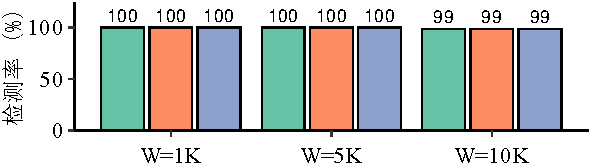
\includegraphics[width=0.66\linewidth]{../pic/featurespy/plot/detection/overall/effectivenessLinux.pdf} &
                    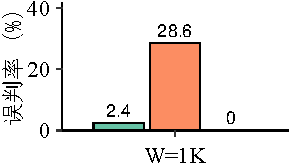
\includegraphics[width=0.33\linewidth]{../pic/featurespy/plot/detection/overall/falsePositiveLinux.pdf}   \\
                    \mbox{\small (a) 检测率}                                                                                &
                    \mbox{\small (b) 误判率}                                                                                  \\
                \end{tabular}
                \caption{Linux数据集中总体检测率和误判率}
                \label{fig:featurespy-expDetectionOverallFalsePositive}
            \end{figure}
        \end{column}
        \begin{column}{.4\textwidth}
            \begin{itemize}
                \item 在对所有窗口大小使用相同检测阈值T时,随窗口大小增大误报率降低(W=5,10\,K时为0)。
                \item {\tt minFeature}方案检测到更多相似数据块,相较于其他两种方案产生更高误报率。
            \end{itemize}
        \end{column}
    \end{columns}
\end{frame}

\subsection{\prototype 原型系统}

\begin{frame}{\prototype 原型系统性能}
    \begin{figure}[!htb]
        \centering
        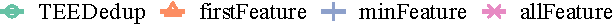
\includegraphics[width=0.7\textwidth]{../pic/featurespy/plot/performance/multiClient/legend.pdf}
        \vspace{5pt}\\
        \begin{tabular}{@{\ }c@{\ }c@{\ }c}
            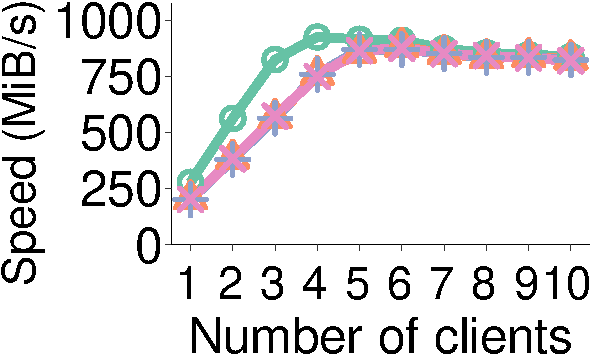
\includegraphics[width=0.32\textwidth]{../pic/featurespy/plot/performance/multiClient/upload_1st_line.pdf} &
            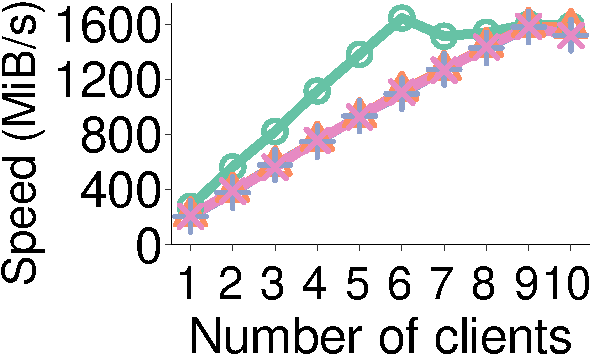
\includegraphics[width=0.32\textwidth]{../pic/featurespy/plot/performance/multiClient/upload_2nd_line.pdf} &
            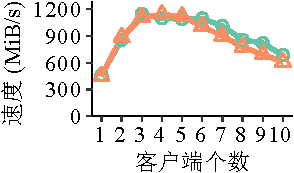
\includegraphics[width=0.32\textwidth]{../pic/featurespy/plot/performance/multiClient/download_line.pdf}     \\
            {\small (a)第一轮上传}                                                                                     &
            {\small (b)第二轮上传}                                                                                     &
            {\small (c)下载}
        \end{tabular}
        \caption{多客户端上传/下载性能。所有\prototype 实例的下载速度均相同的,本文将它们(橙色)与 \sysnameS(绿色)进行比较。}
        \label{fig:featurespy-expMultiClientThroughput}
    \end{figure}

    \begin{itemize}
        \item \sysnameS (4客户端聚合上传速度924.9\,MiB/s)比\prototype 更早达到峰值性能(6客户端聚合上传速度882.2\,MiB/s)
    \end{itemize}
\end{frame}



\section{个人成果}

\begin{frame}[allowframebreaks]{攻读硕士学位期间取得的成果}
    \newcommand{\bstlabelmark}{lo}
    \nocite{*}
    \bibliographystyle{thesis-uestc}
    \bibliography{publication}
\end{frame}

\begin{frame}
    \begin{center}
        {\Huge 衷心感谢老师倾听}

        {\Huge 请各位老师指正!}
    \end{center}
\end{frame}

\end{document}